% TEMPLATE for Usenix papers, specifically to meet requirements of
%  USENIX '05
% originally a template for producing IEEE-format articles using LaTeX.
%   written by Matthew Ward, CS Department, Worcester Polytechnic Institute.
% adapted by David Beazley for his excellent SWIG paper in Proceedings,
%   Tcl 96
% turned into a smartass generic template by De Clarke, with thanks to
%   both the above pioneers
% use at your own risk.  Complaints to /dev/null.
% make it two column with no page numbering, default is 10 point

% Munged by Fred Douglis <douglis@research.att.com> 10/97 to separate
% the .sty file from the LaTeX source template, so that people can
% more easily include the .sty file into an existing document.  Also
% changed to more closely follow the style guidelines as represented
% by the Word sample file. 

% Note that since 2010, USENIX does not require endnotes. If you want
% foot of page notes, don't include the endnotes package in the 
% usepackage command, below.

\documentclass[letterpaper,twocolumn,10pt]{article}
\usepackage{usenix,epsfig,endnotes}
\usepackage{comment}
\usepackage{graphicx}
\usepackage{hyperref}
\usepackage{amsmath}
\graphicspath{ {images/} }

\begin{document}

%don't want date printed
\date{}

%make title bold and 14 pt font (Latex default is non-bold, 16 pt)
%\title{\Large \bf Wonderful : A Terrific Application and Fascinating Paper}
\title{\Large \bf Projecting the AES Encryption on CUDA GPU Framework}

\author{
{\rm Zorawar Moolenaar'20}\\
\rm  Trinity College\\
zsingh@trincoll.edu
%\and
%{\rm Second Name}\\
%Second Institution
}

\maketitle

% Use the following at camera-ready time to suppress page numbers.
% Comment it out when you first submit the paper for review.
% \thispagestyle{empty}


\subsection*{Abstract}
Your Abstract Text Goes Here.  Just a few facts.
Whet our appetites.

\section{Introduction}

%A paragraph of text goes here.  Lots of text.  Plenty of interesting text. \\

% More fascinating text. Features\endnote{Remember to use endnotes, not footnotes!} galore, plethora of promises.\\

Cryptographic algorithms are the underlying principles that facilitate basic human rights like Right to Privacy.
As technology evolves to engage more sensory modalities and more immersive experiences, we are continuously exposing more data about ourselves.
This makes it essential to consume, process and store user-data deliberately and mindfully to prevent abuse that may range from monitoring and censorship to psychological-manipulation and identity-theft.
Thus, services must take-on the onus of protecting the users of their utilities.
At the same time, these services must provide a seamless user-experience. The cost of protection should not be longer wait-times or a worse user-experience in any other form.

One class of cryptographic algorithms used in such a context, are classified under \texttt{symmetric-key cryptography}.
These algorithms provide a modest amount of confidentiality, integrity and reliability within practical computational and temporal constraints.
However, as computational power increases rapidly (in concurrence with Moore's Law, and advancements in high-performance, and quantum-computing based systems), we must re-evaluate the validity of existing algorithms, while also vetting new realisations and concepts.

%Such algorithms rely on computational complexity and hardness to provide the benefits of confidentiality, integrity, and reliability.
% Features like cryptographic hash-functions, symmetric- and assymetric- key crytography, secure random-number generators, together allow 
With increasing availability of GPUs and richer general-purpose GPU (GPGPU) programming paradigms, increasing number of computationally intensive tasks are being re-written to exploit the parallel programming model of GPUs. 

This paper explores a widely used symmteric-key algorithm, the Advanced Encryption Standard~\cite{AES}, endorsed by the National Insitute of Standards and Technology (NIST) in context of GPU computing.  

\section{GPUs and Cryptographic Algorithms}
A cryptographic algorithm is called ``strong enough'' under the assumption that it isn't the weakest link in the system~\cite{strongEnough}.
In practice, \textit{computational hardness} is one feature that contributes to being ``strong enough''.
For secret-key or hashing algorithms this manifests as expanding the number-field for keys and values.
Typically, this requires more computations to calculate (taking away from the user experience), but also making it exponentially harder to break.

Historically, computation costs have been ameliorated this calculation cost, by leveraging dedicated structures: dedicated hardware add-ons such as the MMX instruction set, and hardware-abstracting frameworks such as the OpenBSD Cryptographic Framework. These accelerators offer significant speedup ~\cite{ocf_design}.
The increase in computational power of GPUs has made it more efficient than CPUs at certain tasks, and although they have not typically been used for non-graphics operations, that landscape is changing rapidly thanks to the rise of general-pupose GPU programming paradigm (GPGPU)~\cite{cryptographics}.
Application Specific Integrated-Circuits (ASICs) can be crafted from bottom up tailored to maximise efficiency with respect to some specific algorithm, and simultaneously minimise power consumption~\cite{bhatnagar}.

In such a scenario, what makes GPUs worth examining over the other two options, is that GPUs are more widely available.
They are already present in most modern machines since desktop-managers, web-browsers, video-players, and operating-systems have evolved to leverage the GPU for higher performance.
GPUs offer an excellent trade-off of speed, cost and ubiquity.
Furthermore, algorithms similar to AES are embarrassingly parallel. They perform straightforward mathematical operations on large data-sets --- which GPGPUs are natively designed to tackle.
%Additionally, Cook and Keromytis of Columbia University demonstrate in their book about how GPUs.

However, there are some bottlenecks too.
Operations required by the same algorithm --- such as large-integer modulo and byte shifts --- are very expensive to compute on GPUs~\cite{cuda_pro_guide}~\cite{modulo_error}.
The main performance bottleneck is the overhead of transferring a large amount of data to the GPU to operate upon.
Consequently, older versions of GPU architecture did not provide significant performance gain; however, with optimisations such as stream processing and exploiting memory techniques (coalescing, constant, shared) have yielded a substantial speed-up~\cite{iwai}.

\section{The Advanced Encryption Standard}
In Late 1997, in response to exposed vulnerabilities of the Data Encryption Standard (DES) --- the then federal standard ---, the National Institution for Standards and Technology (NIST) called for proposals of an Advanced Encryption Standard (AES) to replace DES.
NIST received fifteen proposals of candidate ciphers, which included algorithms authored by IBM (who developed DES), by Ron Rivest, and among others by Dutch Cryptographers, Vincent Rijmen and Joan Daemen.
In 2000, NIST accepted a variant of the Dutch algorithm, called Rijndael.
Around 2002, it became the federal standard for classified to top-secret US government communication.
AES has become of the most important algorithms today: it is used to encrypt WiFi pre-shared keys, in routers, for HTTPS/TLS security by webservers used in banking, commerce, privacy-oriented and other websites.

Especially in context of web-servers, AES serves a dramatic computational overhead~\cite{ieee_cuda}. Webservers have to deal with millions of requests, and an addition handle encryption/decryption via the openssl library.
The implementation structure of AES exhibits a high degree of data parallelism, and so CUDA's single-instruction multiple-data architecture lends itself natively.
Theoretically, AES is an extra burden for webservers. 
If it could be repurposed to be delegated to GPUs, webservers will see accelerated performance and security.

\subsection{Algorithm Overview}
AES operates on a 4x4 \textit{state} matrix, the input and output data, using galois (finite) field operations.

The state represents 128-bits \textit{block} of the data to be encrypted or decrypted.
It also consumes a \textit{cipher key} of {128-bits}, {192-bits} or {256-bits}, conducts 10, 12 or 14 \textit{rounds} of execution (i.e., repititions of transformation).
The same cipher key is used for both encryption and decryption. AES is hence considered a \textit{symmetric-key} algorithm.
Like most commercial applications, the included implementation uses a cipher key of 128-bit length.

The algorithm begins with \textit{key-expansion}, a routine to generate \textit{round keys} from the given cipher keys.
Then, AES performs four different byte-oriented transformations in each round:
\begin{enumerate}
    \item \textit{Byte Substitution} using a substitution matrix; this provides \textit{confusion}~\cite{shanon}
    \item \textit{Shifting Rows} of the state matrix by some fixed offset
    \item \textit{Mixing Columns} of the state matrix; this together with row-shifting provides \textit{diffusion}~\cite{shanon}
    \item \textit{Key Addition} of the \textit{round key} to the state matrix
\end{enumerate}

Step 1. provides \textit{confusion}, and step 2. and 3. provide \textit{diffusion}; together, these steps make AES a secure operation and make it harder to perform cryptanalysis~\cite{shanon}.
It is worth noting that in the last round of transformation, column-mixing is not performed.

The details of the implementation of each step of the process have been heavily documented in the source code in a readable, and concise yet expressive manner. This not only remarkably cuts-down the length of this paper, but makes the algorithm easier to understand. 

\section{Source-Tree}
This implementation is composed of four \texttt{c-source} files, and one \texttt{header} files.
\begin{enumerate}
    \item \texttt{main.cu}: contains CUDA/C implementation of AES, with IO and print utilities
    \item \texttt{keygen.c}: generates a random 128-bit key that each iteration of AES may use
    \item \texttt{gen\_payload.c}: generates an obscure payload of random characters to fill-up N bytes of data. Possible values for this implementation: 8Mib, 16Mib, $...$, 1024MiB
    \item \texttt{utils.c}: common utilities used by all applications
    \item \texttt{aes.h}: signatures and constants required for the application
\end{enumerate}

\section{Benchmarks}
\subsection{Testing Environment}
Tests have been conducted on Trinity College's \texttt{pine} server, access to which was graciously provided by Dr. Peter Yoon. This server housed both, the CPU and GPU used to test both versions of AES.

The CPU version of AES falls back on the native openSSL implementation --- which ships with many GNU/Linux distributions, including the host Operating System, Ubuntu 16.04. Calculations were performed using twenty-four 64-bit Intel Xeon CPUs, clocked at 1.95GHz with 2 threads per core. (results were gathered using \texttt{lscpu}).

The CUDA/C implementation of AES runs on an NVIDIA Tesla GPU with 65K of constant memory, about 50K of shared memory, and 12GB of global memory. 

\subsection{Results}
As visible in the graph, the GPU implementation by far outperforms CPU-based AES. In fact, graph hints that the CPU v. GPU time eventually follows parallel lines. The tests were also conducted on an older GPU: while timing for small-sized payloads were much closer than in Figure \ref{Tesla}, there was still a siginifcant gap. The parallel trend was apparent in this test too.

\begin{align}
    S(n,p) &= \frac{
            T_{serial}(n)
            }{
            T_{parallel}(n,p)
            }
    \\
    S(512, p) &= \frac{
            3.208
            }{
            0.0454
            }
    \\
    S(512, p) &= 70.66
\end{align}

Hence, the GPU implementation shows a 70.66 times speedup.

\begin{figure}
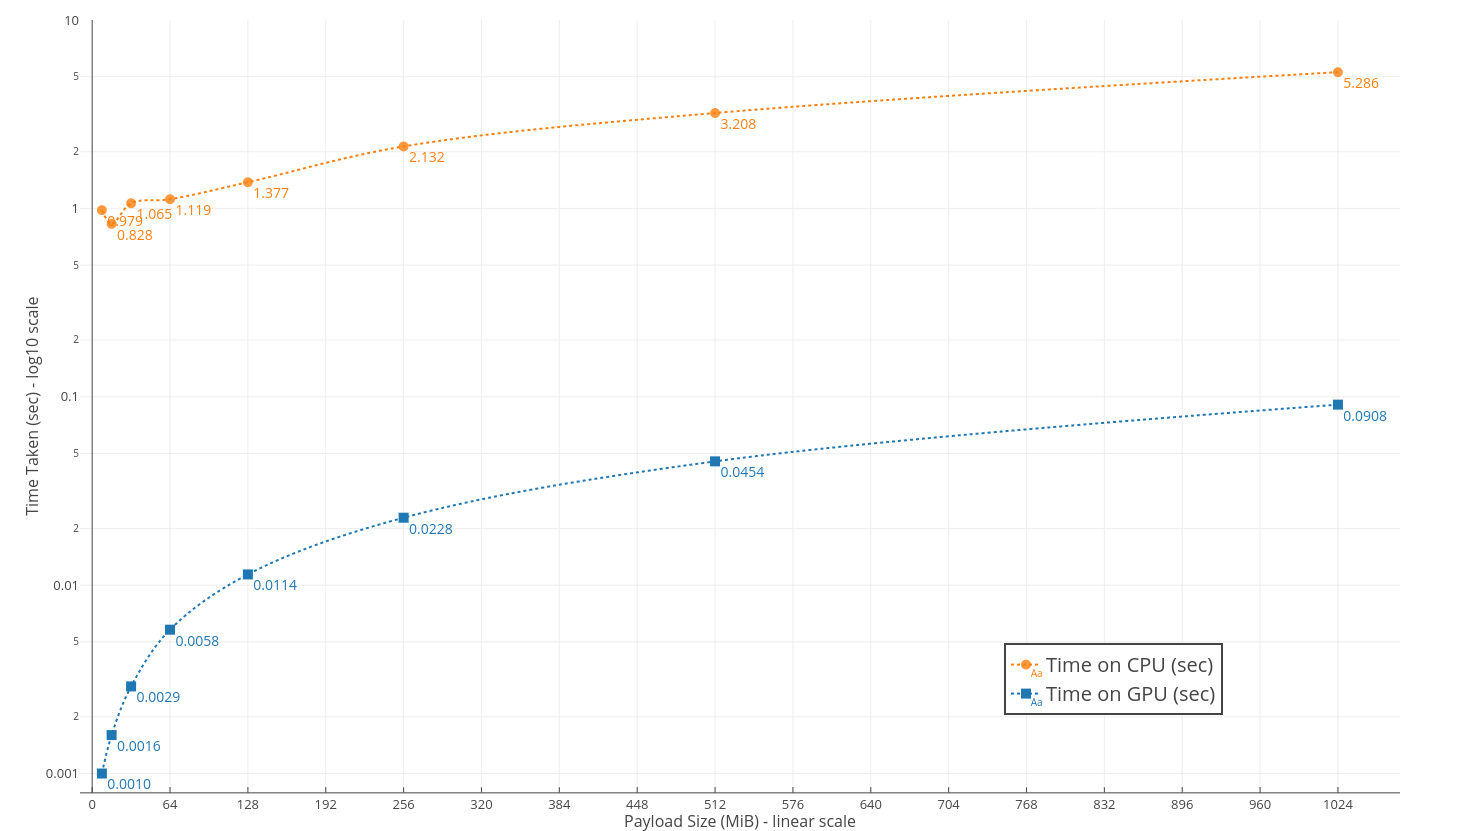
\includegraphics[scale=0.16]{HPC}
\label{Tesla}
\caption{
    Payload Encryption Time
    \endnote{
        A clearer, interactive version of the graph may be found at
        \href
        {https://plot.ly/~zorawar87/1/}
        [https://plot.ly/~zorawar87/1/]
    }
}
\end{figure}

\section{Future Work}
While the results are conclusive in pointing the superiority of a GPU-based encryption system, the project does not implement a working decryption utility. While in theory this was simple, in practice, there were some errors that could not have been fixed in the current iteration.

It is worth noting that the implementation heavily relies on fighting the performance bottleneck of memory transfer. Consequently, appropriate constant matrices are placed in the device constant matrix. It also makes use of shared memory when dealing with the state matrix, and computations keep in mind principles of warps, memory coalescing and DRAM  bursts.

One claim that may be worth investigating, is that rather than using constant substitution matrix and round-constants, they should be calculated on the GPU, since matrix multiplication is a trivial problem of parallelisation. Unfortunately, even though I spent a lot of time trying to understand the surrounding math, it is beyond the scope of what I can make sense of at this time.

\section{Reflections, Challenges \& Limitations}
The most time consuming part of this project was actually understanding the internals of the AES algorithm. Once I got a sense of how the implementation might be composed, I learned how to use a debugger (\texttt{cuda-gdb}), and finally grasped the pertinent concepts and the ability to follow through a single application run.

Additionally, I expanded what I knew about \LaTeX typesetting, by using style file and learning to use \textsc{Bib}\negthinspace\TeX  for citation management; representing data using charts using \texttt{plotly}, and \texttt{make} to simplify the general software development workflow.

{\footnotesize \bibliographystyle{acm}
\bibliography{cuda-aes}}

\theendnotes

\end{document}
